% Author: Till Tantau
% Source: The PGF/TikZ manual
\documentclass{article}

\usepackage{tikz}
\usetikzlibrary{mindmap,trees}
\begin{document}
\pagestyle{empty}
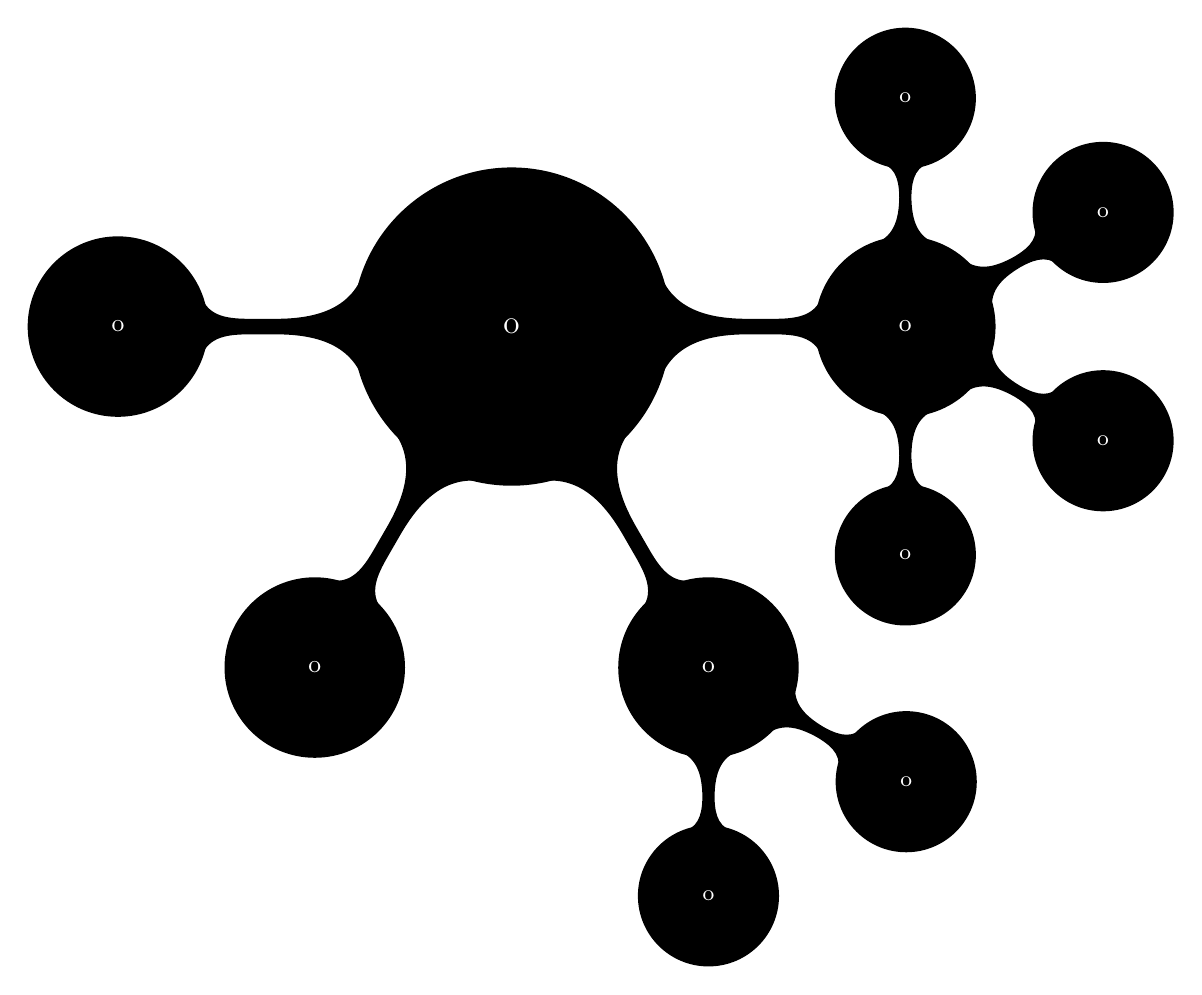
\begin{tikzpicture}
  \path[mindmap,concept color=black,text=white]
    node[concept] {o}
    [clockwise from=0]
    child[concept] {
      node[concept] {o}
      [clockwise from=90]
      child { node[concept] {o} }
      child { node[concept] {o} }
      child { node[concept] {o} }
      child { node[concept] {o} }
    }  
    child[concept] {
      node[concept] {o}
      [clockwise from=-30]
      child { node[concept] {o} }
      child { node[concept] {o} }
    }
    child[concept] { node[concept] {o} }
    child[concept] { node[concept] {o} };
\end{tikzpicture}\end{document}
